\documentclass[a4paper, 11pt]{article}
\usepackage{comment} % enables the use of 
\usepackage{fullpage} % changes the margin
\usepackage[justification=centering]{caption}
\usepackage[figurename=Fig.]{caption}
\usepackage{graphicx}
\usepackage{subfigure}
\usepackage{float} 
\usepackage{wrapfig} 
\usepackage{hyperref}

\begin{document}
%Header-Make sure you update this information!!!!
\noindent
\large\textbf{COMP532 Assignment 2} \hfill 
\normalsize Deep Reinforcement Learning \hfill  
\\\\

\section*{Setup}
%\includegraphics[width=0.5\textwidth]{hand.png}[1.19]
$\bullet$ State chosen game: I chose Atari Breakout-v4 which is quite popular applying Deep-Q Learning Network. 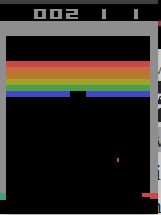
\includegraphics[height=5cm]{game.png}\\
Firstly, we can play around to get information from breakout-v4. We can observe direction, velocity of the ball in two consecutive frames, but in order to overcome the game we need to keep 4 frames to get the acceleration as a single observation.
Atari environment outputs 210x160x3(RGB) arrays we want machine could observe by itself, and also reduce the size of input to acceleration training. Therefore I decide to resize to 80x80x3 and convert to gray-scale 80*80*1 because hit which color is not matter for us to win this game. I keep 4 frames then send to network.\\
$\bullet$ Network Structure:\\
Input: 80x80x4\\
Convolutional layer1: 32 filters of 8 x 8 with stride 4 with the input image.\\
Convolutional layer2: Convolves 64 filters of 4 x 4 with stride 2.\\
Convolution layer3: Convolves 64 filters of 3 x 3 with stride.\\
Fletten Layer\\
Fully-Connected: consists of 512 rectifier units.\\
Output: Output layer is a fully-connected linear layer with a single output for each valid action.\\
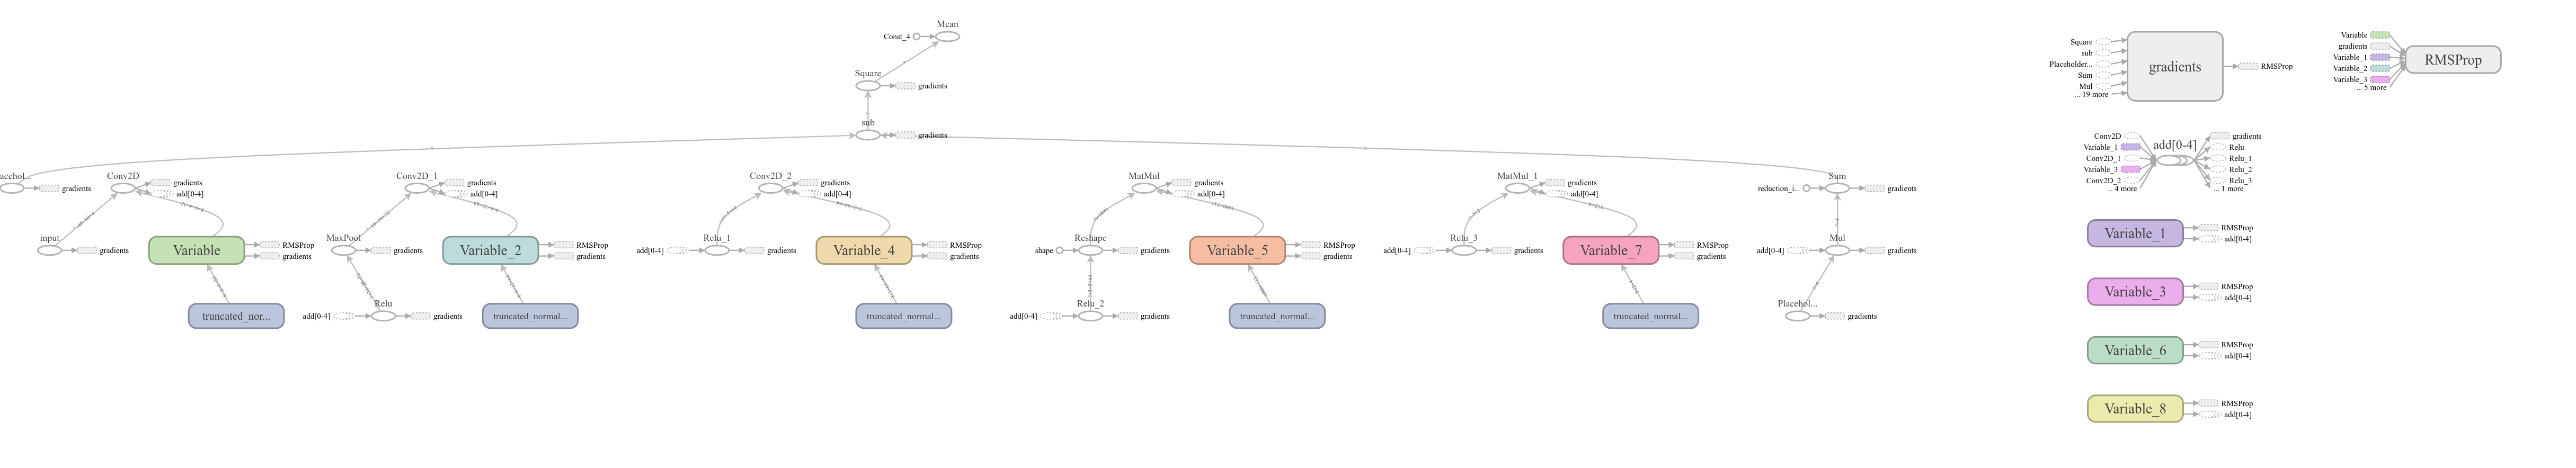
\includegraphics[width = 20cm]{graph.png}
%\includegraphics[width=0.5\textwidth]{clean.png}


\section*{Results}
In this section, I record part of results which are not good when I were testing and optimizing game. In the beginning, I used Adam optimizer which let agent could not learn very well. Updating $\epsilon$ too frequently, small memory buffer and improper initial values caused model couldn't converge and learn.
\subsection*{Optimizer}
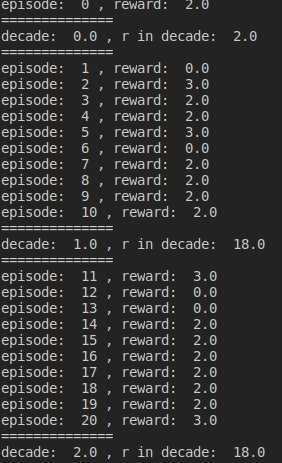
\includegraphics[height = 5cm]{adam1.png}
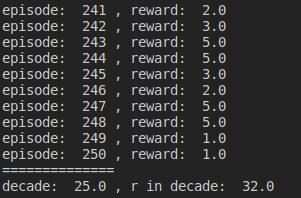
\includegraphics[height = 5cm]{adam3.png}
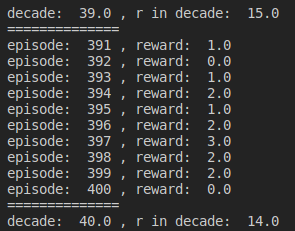
\includegraphics[height = 5cm]{adam2.png}\\
tf.train.AdamOptimizer(0.001).minimize(self.cost) tensorflow adam optimizer with learning rate 0.01. Because the result was quite bad I terminated in 500 episode. I observed the max reward only to 32 after that the performance decreased. Adam can be looked at as a combination of RMSprop and Stochastic Gradient Descent with momentum. Adam retains Momentum's gradient speed adjustment for the direction of the past gradient and Adam's adjustment of the learning rate of the square of the past gradient. In addition, Adam has the "offset correction" for the parameters, so that each learning rate will be determined. The scope will make the parameter update more stable. Stability is the main reason I used Adam, because in some tutorial I saw the curve is turmoil. I tried learning rate(0.0001 or less) but the results still are unpleasant. \\

tf.train.RMSPropOptimizer(0.00025,0.99,0.0,1e-6).minimize(self.cost)\\
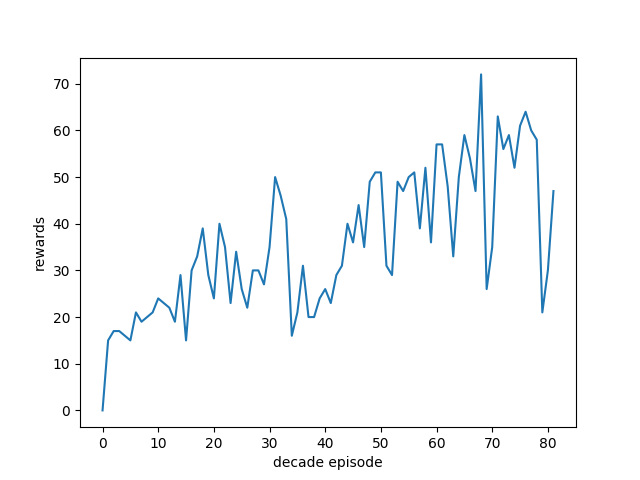
\includegraphics[height = 5cm]{81.png}
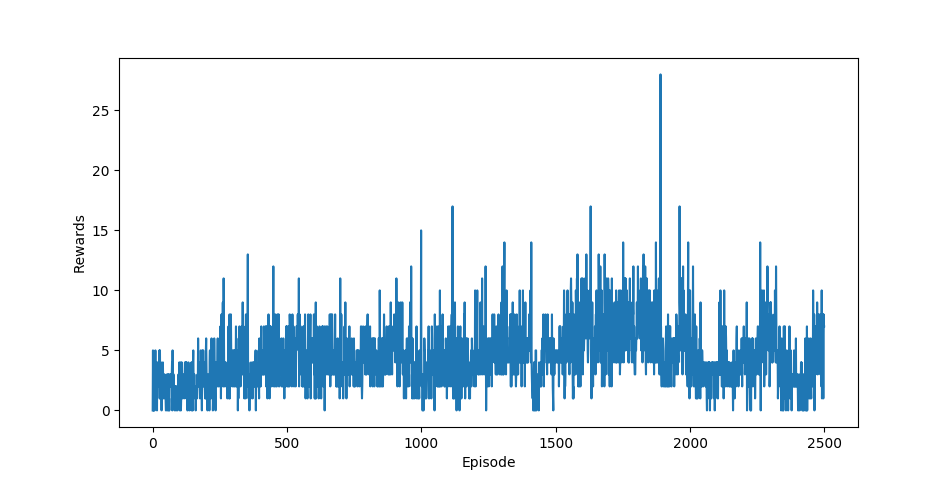
\includegraphics[height = 5cm]{longer.png}\\
The left graph plotting to 810 episode with rewards. We can observe the overall trend is going up. In the beginning, the paddle is static through the learning model can move paddle giving response. The right graph with higher training time and plot every run. If we check each run the trend slightly goes up, but check each decade can have more obvious result.
\subsection*{Turing Parameters}
Creating a buffer queue data type to store (cur\_state, actions, reward, next\_state, done) information, which apply in the replay however if set too low, when queue is full some value-able leaned information may be pop out. Applying de ep learning q network I update $\epsilon$ base ob learning steps(time) Due to I'm using $\epsilon$ greedy, the balance between exploitation and exploration depend on $\epsilon$ value. The best decreasing value would be (MAX - MIN)/STEPS, we can observe from below images. The left image is using higher decreasing epsilon(0.0001) the right image use(0.00009) both same buffer size and steps.\\
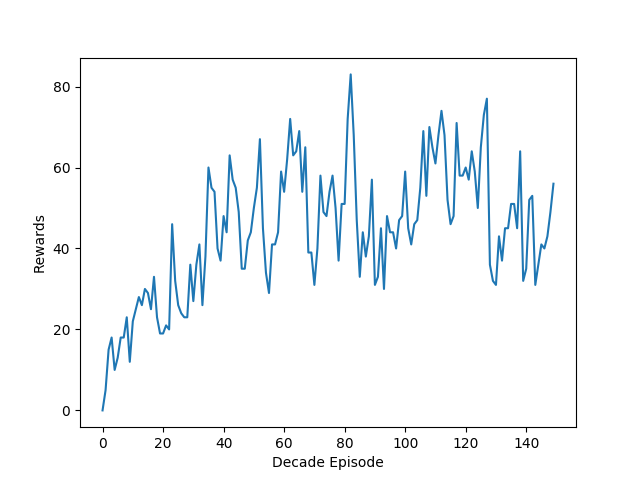
\includegraphics[height = 5cm]{decases.png}
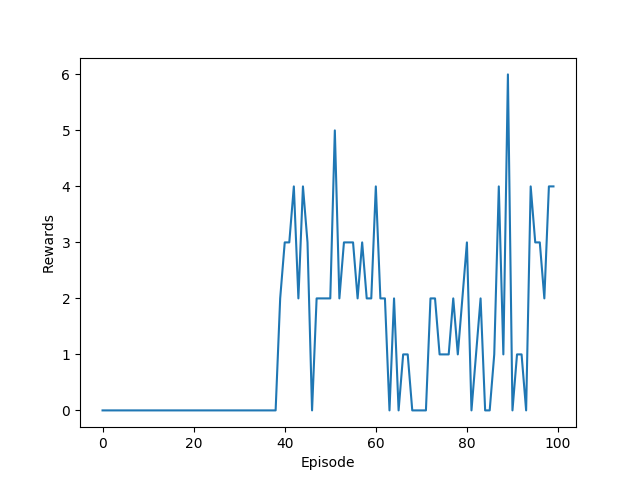
\includegraphics[height = 5cm]{test.png}\\
There are short training result graphs with different updating epsilon frequency and steps. I set $\epsilon$ default value is 1.0 that means 100\% doing exploration in beginning. And we update $\epsilon$  base on observation and min $\epsilon$ is 0.1 so model won't totally do exploit in the end. The graphs showing the $\epsilon$-greedy feature, the model almost does exploration seldom exploit learned. Left image with less decreasing $\epsilon$ value right image with higher value and steps means more opportunities do exploit learned.\\
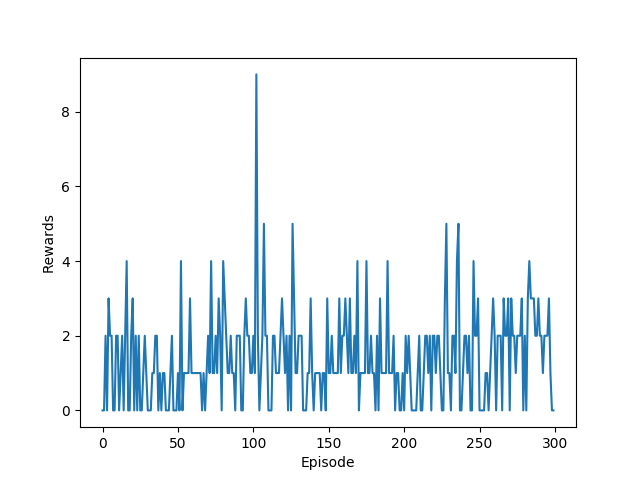
\includegraphics[height = 5cm]{low.png}
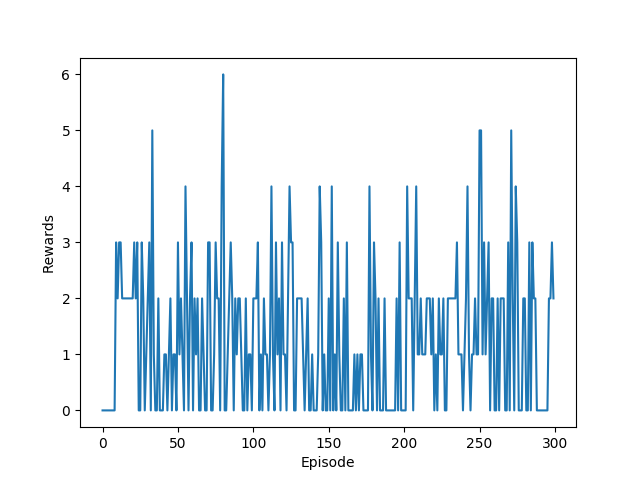
\includegraphics[height = 5cm]{higher.png}
\subsection*{Conclusion}
My model trains on tensorflow cpu(intel 16 cores), the network compare VCC16 and other DeepNetworks is tiny, the Experience replay to find the optimal solution let training take times and each training starts with a uniformly random policy; However, DQN with Prioritized replay can make efficient use of these infrequent rewards and learn them. So Prioritized replay will end each episode faster. Furthermore, there is another Network is DualDeepQnetwork which splits the Q of each action into the value of state plus the Advantage of each action. In the future work those methods could improve overall performance.






\end{document}
